\part{De l'annonce à l'emploi:  rôle et place des répondants, des intermédiaires et de l'adresse dans les \textit{Affiches}}


\chapter{Répondants et certificat: l'importance de la cooptation et des réseaux d’information}

Une partie essentielle des annonces, peut-être la plus importante aux yeux des domestiques qui les écrivent, a pour l'instant échappé à l'analyse: il s'agit de l'adresse, toujours placée en fin d'annonce, et dont l'étude révèle beaucoup au sujet des liens et des processus sociaux à l'œuvre dans la recherche d'emploi au XVIIIè siècle. 

Mais avant même de mentionner une adresse ou un intermédiaire, les annonces mettent en avant des références, des individus susceptibles d'informer un potentiel employeur des qualités et de l'honnêteté du ou de la domestique. Complémentaire de la mise en valeur de sa propre personne ou de son labeur, la mention des "bons répondants" fait écho à l’importance des réseaux informels dans la recherche de travail au XVIIIè siècle. Garants à la fois de sérieux et de bonnes mœurs, les répondants ne concernent pas seulement le travail domestique: ils sont également nécessaires dans certaines manufactures, pour rejoindre un atelier ou une communauté de métier\footcites[p.86-87]{crowstonFabricatingWomenSeamstresses2001}, et même dans les ateliers de filature mis en place sous la Révolution pour fournir du travail aux plus démunies\footcites[p.43]{dicaprioOriginsWelfareState2007}. Mais la référence dans la domesticité, où travailleurs et travailleuses sont soumis à une méfiance de tout instant parce qu'ils pénètrent l'espace privé du maître et se voient accorder sa confiance, est primordiale. Dans la seconde moitié du XVIIIè siècle, où la défiance de la noblesse et de la bourgeoisie envers les classes laborieuses croît encore, elle devient indispensable. Elle se double même d'un mode de référencement institutionnel, avec l'apparition du certificat dès le XVIè siècle\footcites{guttonDomestiquesServiteursDans1981}, dans lequel les domestiques ont obligation de consigner le contact de leurs anciens employeurs, voire d'obtenir leur accord écrit avant de prendre congé. Loin d'être répandu, le certificat représente néanmoins un moyen fort de régulation du travail ancillaire, notamment aux yeux de la police urbaine. 

Dans le cas des petites annonces, ces répondants et leur rôle de "médiatisation de la confiance\footcites{kramplAdresserClercHuissier2017} sont d'autant plus importants qu'on s'éloigne des réseaux traditionnels de l'embauche que sont le voisinage, l'interconnaissance, la clientèle, la recommandation par un domestique déjà dans la maison ou par un proche. Ainsi, loin de subvertir ou de supplanter les logiques et procédures instituées de l'Ancien régime et favorables aux maîtres, le nouveau support que représente l'annonce semble à première vue plutôt s'y conformer.



\section{Méthode}

Ayant pu observer que les formes de recommandations contenues dans les annonces sont très régulières et adoptent des formules qui varient peu dans le temps ou selon la ville, j'ai eu recours pour les extraire à des expressions régulières. J'ai d'abord noté que le mot privilégié dans les annonces est "répondant", le plus souvent employé dans la formule "[Le domestique] fournira de bons répondants". Il a ensuite fallu prendre en compte les possibles variations typographiques ou erreurs d'océrisation ("e" accentué ou non, présence d'un "t" ou non à la fin du mot), ainsi que les possibles coupures du mot en fin de ligne. J'ai ensuite pu ajouter une colonne à mon \textit{dataframe}, précisant cette fois simplement si l'annonce contient ou non l'expression régulière.

Afin de m'intéresser aux possibles qualificatifs appliqués aux répondants, j'ai en outre extrait, à partir des textes des annonces, les bigrammes et trigrammes qui contiennent le mot répondant, que j'ai également ajoutés au \textit{dataframe}.

Pour ce qui est du certificat, j'ai employé la même méthode, à partir de l'expression \fbox{cer-?ti-?fi-?ca}.


\section{"De bons répondants": une mention essentielle des annonces}

L'expression ainsi élaborée, \fbox{re?é?-?pon-?dan}, m'a finalement permis de constater que plus d'une annonce sur cinq contiennent une référence aux répondants (1151 sur 5064). Parmi elles, plus des trois quarts (930 annonces) précisent avoir de "bons" ou "les meilleurs" répondants. 

Par ailleurs, la mention des répondants semble assez peu impactée par la variable de genre: un peu moins d'un tiers des annonces déposées par des femmes sont concernées, contre un quart pour les hommes. Étant donné les limites de la catégorisation sexuée dans le corpus, et le fait que la majorité des annonces n'ont pu être classées, je considère que cette différence est assez négligeable. 


\begin{figure}[h]
	\centering
	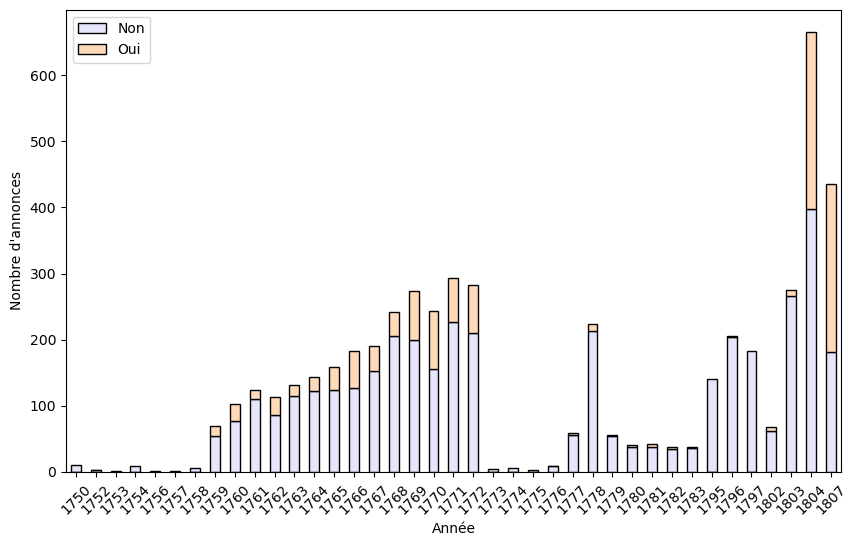
\includegraphics[width=12cm]{hist_rep_chrono.png}
	\caption{Répartition de la mention des répondants selon le temps}
\end{figure}

Enfin, la présence ou non des répondants dans l'annonce évolue au cours du temps: si les annonces "avec répondants" réprésentent entre un dixième et un quart des annonces dans les années 1760 et 1770, elles sont plus d'un tiers en 1804, et plus de la moitié en 1807. 

En comparaison, la présence du certificat dans les annonces est beaucoup plus rare, et finalement proportionnel à son impact réel sur le monde de la domesticité: seules 199 annonces le mentionnent.


\chapter{"S'adresser à ...". Intermédiation, modes d'adressage et capacités d'agir des domestiques}

Si l'omniprésence des références et des répondants dans les annonces est un indicateur du maintien et de la persistance de logiques de cooptation et de recherche d'emploi spécifiques à l'Ancien Régime, le journal d'annonces ne peut pas être analysé uniquement comme un moyen parmi d'autres de trouver un travail. En proposant un nouveau support, les \textit{Affiches} proposent également de potentielles nouvelles stratégies et manœuvres à disposition des domestiques: "la petite annonce pose ainsi la question de l’articulation entre ce nouveau support et la problématique exigence d’un "travail de confiance" inhérent aux relations laborieuses\footcites{kramplAdresserClercHuissier2017}". 


\section{Méthode}

L'adresse est probablement la partie la plus uniforme et la plus stable dans le temps de l'annonce. C'est cette régularité qui m'a permis de l'inclure parmi les catégories de \textit{spans} à extraire avec le modèle entraîné sur Spacy; de la même façon qu'avec les compétences ou les emplois, un peu plus de 500 annonces ont été annotées en vue de l'entraînement.  

Au final, ce sont 1184 annonces pour lesquelles le modèle a permis d'extraire une adresse. 


\section{Intermédiaires et adresses: aperçu du réseau urbain de l'information}

L'extraction de l'adresse des annonces aurait pu donner lieu à une tentative d'esquisse de la géographie domestique à l'aide de techniques de spatialisation de l'information. Ayant manqué de temps pour mener à bien ce projet dans le cadre de ce mémoire, je présente ici quelques pistes de réflexion autour des modes d'adressage et des intermédiaires des petites annonces, largement inspirées de l'article qu'Ulrike Krampl a dédié à la question\footcites{kramplAdresserClercHuissier2017}. 

Tout d'abord, le mode d'adressage signalé au sein des annonces est en très grande partie implicite; "s'adresser à" signifie conventionnellement s'adresser à l'oral, en personne, si bien que seules onze annonces du corpus précisent "s'adresser verbalement" ou "de vive voix". Certaines indiquent néanmoins les heures auxquelles on peut les trouver chez eux:  "S'ad. verbalement, le matin jusqu'à 2 heures, chez Madame S. D., rue St.-An-toine, n. 58, maison de l'épicier, en face du théâtre Mareux\footnote{\textit{Affiches de Paris}, 13 mars 1807}". 63 annonces, en revanche, précisent qu'il faut répondre à l'annonce par écrit ou par lettres, et le plus souvent franc de port. 

Dans son article, Ulrike Krampl remarque que trois types d'adresses peuvent être indiquées par les domestiques: "celle du bureau, celle des particulier.es concerné.es et celle d’intermédiaires". Dans ce corpus, les annonces qui renvoient à un bureau d'adresses (du journal ou autre) sont très minoritaires: je n'ai pu en retrouver que 109, toutes parues dans les années 1760 à Lyon ou entre 1804 et 1807 à Paris. La pratique majoritaire semble donc être le renvoi vers son adresse particulière ou l'adresse d'un ou d'une intermédiaire, la différence entre les deux étant d'ailleurs difficilement perceptible dans les annonces.

En outre, Ulrike Krampl s'intéresse dans son article à la sociologie du groupe des intermédiaires. Elle remarque que ceux-ci sont en grande partie voire en majorité des officiers publics, hommes de droit ou de l'administration dont le rôle de médiation entre individus est déjà attesté dans d'autres sphères que la presse, et qui répondent au besoin de contrôle et d'institutionnalisation des \textit{Affiches}. Néanmoins, cette configuration marquée par un processus de "judiciarisation" des annonces ne semble pas se retrouver dans ce corpus: parmi les métiers du droit et de la justice signalés par l'historienne (procureur, huissier, clerc et commis, ...), je ne retrouve que les notaires, qui demeurent très rares avec 12 occurrences, et un unique avocat. En revanche, d'autres professions, signalées par U. Krampl mais définies comme marginales, se retrouvent beaucoup plus dans mon corpus: les portiers notamment, dont l'historienne ne retrouve que quatre occurrences (3,4\% de son corpus, et uniquement dans des offres d'emploi), sont ici au moins au nombre de 87, soit plus de 7\%. Les marchands quant à eux, se retrouvent dans des proportions assez similaires entre les deux corpus: ils sont les intermédiaires de 6,7\% des annonces chez Ulrike Krampl et de 5,2\% des annonces ici.

Enfin, l'étude du genre des intermédiaires corrobore également les observations générales de l'article: l'intermédiation est majoritairement une activité d'hommes, mais où les femmes peuvent se faire une place. Elles sont même un peu plus présentes dans mon corpus, passant de 9,4\% des intermédiaires chez Ulrike Krampl à près de 30\% des annonces qu'il m'a été possible de genrer (197 femmes sur 667 annonces). 


\section{“On ne recevra pas de lettres des petits bureaux”: l'annonce comme alternative au marché traditionnel du travail?}

Parmi les annonces et les formules d'adressage, une phrase revient dans plusieurs dizaines d'annonces: "On ne recevra pas les lettres des petits bureaux". Cette formule fait référence aux bureaux de placement, un nouveau mode d'intermédiation et de recherche de travail, qui apparaît au XVIè siècle, comme l'annonce, dont il est l'un des premiers émetteurs. Les bureaux ont la particularité au XVIIIè siècle de tenir des registres de domestiques, qui se veulent autant des outils de centralisation de l'information que de régulation et de contrôle de l'activité ancillaire: à partir des témoignages de leurs anciens maîtres, ils indiquent les bonnes et mauvaises qualités des domestiques, les maisons qu'ils ont servies et tout renseignement qui pourrait intéresser un potentiel employeur, lequel a parfois d'ailleurs droit à une "période d'essai" avec le valet ou le serviteur recommandé par le bureau\footcites{sabattierChapitreConditionDomestique1984}. 

Si, dans les faits, les bureaux de placement ont un impact très limité par rapport à l'importance des réseaux informels de cooptation et d'intermédiation au XVIIIè siècle (ils sont au nombre de deux ou trois à Paris à la fin du siècle), ils semblent faire l'objet de nombreux reproches de la part des domestiques en recherche d'emploi, peut-être du fait de leurs techniques commerciales agressives ou de leur taux de succès limité, en témoigne cette annonce publiée à Paris en mars 1804: "Un citoyen d'un âge mûr, sachant raser, coëffer, faire une petite cuisine en cas de besoin, le service de la chambre et de la table, panser let chevaux, mener un cabriolet, desire se PLACER à Paris ou à la campagne. Il est muni de bons certi-ficats et a de bons répondans. S'adres. à Mad. Roytel, mar-chande limonadiere, rue Joubert, n. 515, Chaussée d'Antin, pour remettre au cit. Baptiste. On ne recevra pas de lettres des petits bureaux qui prétendent donner des places\footnote{\textit{Affiches de Paris}, 30 mars 1804}"
Ces références aux bureaux de placement restent marginales dans le corpus d'annonces, mais elles donnent certains indices sur la façon dont les individus naviguent au milieu des différents supports et réseaux qui sont à leur disposition pour trouver du travail, et qui se multiplient à l'ère de la presse de grand tirage. L'anonymat permis par l'annonce, notamment, représente un changement important par rapport aux siècles précédents. Les précisions apportées par certains demandeurs, qui souhaitent qu'on s'adresse à tel commerce ou telle maison "sans (...) dire le sujet\footnote{\textit{Affiches de Paris}, 30 mars 1804}" de sa demande ou sans "faire aucune question au portier\footnote{\textit{Affiches de Paris}, 19 mars 1804}", permettent d'envisager les journaux d'annonces comme permettant une marge de manoeuvre vis-à-vis des réseaux traditionnels du travail domestique, notamment lorsqu'on souhaite trouver un nouvel emploi sans en informer ses maîtres ou ses proches. Une perspective déjà évoquée par Clyde Plumauzille et Ulrike Krampl\footcites{kramplPresseAnnoncesParisienne2020}: l'annonce devient alors "un outil émancipatoire par rapport aux logiques de contrôle inhérentes à l’interconnaissance, à la recommandation et au bureau de placement". 

\bigskip

Ainsi, si les demandes d'emploi dans la presse montrent de nombreux signes de la persistance de logiques de cooptation spécifiques à l'Ancien régime (en premier lieu, l'importance des référents et des garants), elles donnent également des indices sur les façons dont les individus se saisissent de supports inédits pour former des stratégies face à un marché qui leur est défavorable, et où peut parfois s'exprimer une capacité d'agir nouvelle.
